\chapter{Planteamiento del Problema}
    El planteamiento del problema debe ser dividido en base a:

    \begin{itemize}
        \item \textbf{Descripción u contexto:} 3 u 4 líneas
        \item \textbf{Macrocontexto:} 1.5 páginas (Contexto más general - puedes verlo como el nivel mundial,  aunque no simboliza ello)
        \item \textbf{Mesocontexto:} 2 páginas (Contexto algo más específico - Podrías verlo como un contexto nacional u regional, aunque no simboliza ello)
        \item \textbf{Microcontexto:} 2.5 páginas (Contexto totalmente específico y exacto del tema - Podrías verlo como un contexto directo de tu tema, en la institución o demás)
        \item \textbf{Párrafo conclusivo del problema} (remembranza del planteamiento y una conclusión del mismo) => establece la naturaleza y la dimensión del problema, así como la importancia de la solución
    \end{itemize}

    \textbf{Párrafo de contexto del trabajo}. Lorem ipsum dolor sit amet consectetur adipisicing elit. Voluptate dolor sapiente accusamus vel tempore distinctio dicta architecto at beatae aliquam, cumque consequatur iure, aspernatur unde ratione a enim non molestiae voluptas nemo. Enim sed laudantium repellat odit eligendi quam facilis perspiciatis similique quo impedit praesentium eos error et corrupti quidem, aperiam consequuntur debitis libero tempora commodi aut voluptatum? Quasi numquam temporibus, tempore amet commodi tempora, mollitia hic esse molestias earum eligendi, sint rem suscipit! Quia est veritatis aspernatur nihil, eius consectetur tenetur quaerat, sunt quo numquam nesciunt ipsam iure reiciendis quisquam facilis totam obcaecati rem, culpa praesentium voluptates voluptatum sit. 

    \begin{figure}[H]
        \centering
        %\isPreprints{\centering}{} % Only used for preprints
        \caption{Una investigación nunca termina, solo se ve limitada por nosotroso
        \label{fig-contexto-investigacion}}    
                
        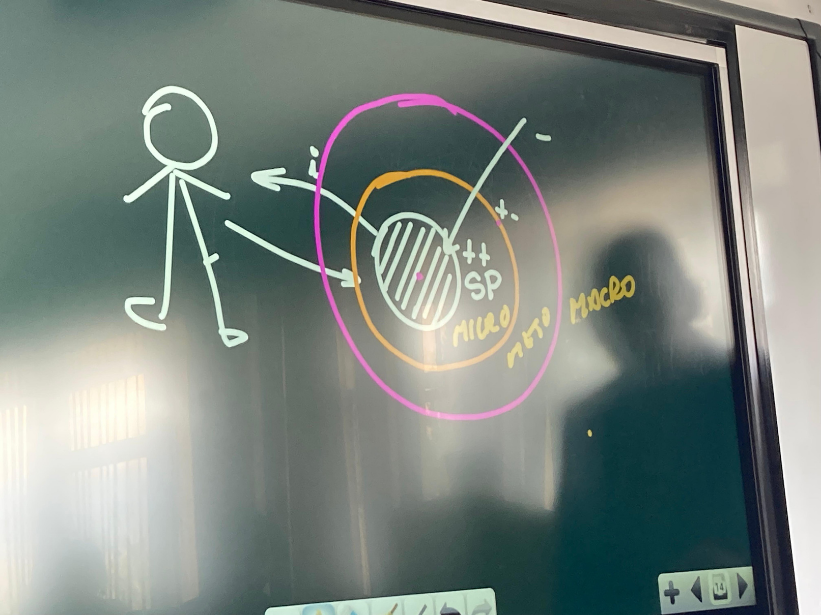
\includegraphics[width=6.0 cm]{src/imgs/nivel-contexto-investigacion.png}

        \vspace{0.1cm}
        % \small EN CASO DE SER BAJO ELABORACIÓN PROPIA, NO HACE FALTA AGREGAR LA NOTA
    \end{figure}
% --- RELLENAR ---
 % Los paréntesis en las secciones deben ser eliminados
\section{Primera sección (Macrocontexto)}
    \begin{sectext}
        Lorem ipsum dolor sit amet consectetur adipisicing elit. Voluptate dolor sapiente accusamus vel tempore distinctio dicta architecto at beatae aliquam, cumque consequatur iure, aspernatur unde ratione a enim non molestiae voluptas nemo. Enim sed laudantium repellat odit eligendi quam facilis perspiciatis similique quo impedit praesentium eos error et corrupti quidem, aperiam consequuntur debitis libero tempora commodi aut voluptatum? Quasi numquam temporibus, tempore amet commodi tempora, mollitia hic esse molestias earum eligendi, sint rem suscipit! Quia est veritatis aspernatur nihil, eius consectetur tenetur quaerat, sunt quo numquam nesciunt ipsam iure reiciendis quisquam facilis totam obcaecati rem, culpa praesentium voluptates voluptatum sit. 

        \begin{table}[!ht]
            % \centering
            \small % Un punto menos ayuda a la legibilidad en tablas densas
            \renewcommand{\arraystretch}{1} % Espacio equilibrado entre filas
            
            \caption{Atributos negativos frecuentemente asociados con las arquitecturas de pantallas volumétricas.}
            \label{tab:atributos-negativos-pantallas}

            % Usamos tabularx para que la tabla se ajuste exactamente al ancho de página
            \begin{tabularx}{\textwidth}{@{} >{\raggedright\arraybackslash\bfseries}p{3.5cm} X X @{}}
                \toprule
                \textbf{First Header} & \textbf{Second Header} & \textbf{Third Header} \\ 
                \midrule
                First Part & Second Part & Third Part \\
                \addlinespace[0.3cm]
                
                First Part & Second Part & Third Part \\
                \addlinespace[0.3cm]
                
                First Part & Second Part & Third Part \\
                \bottomrule
            \end{tabularx}
            
            \noindent{
                \footnotesize{
                    \textit{Nota.} Adaptado a partir de ...
                }
            }
    \end{table}

        Lorem ipsum dolor sit amet consectetur adipisicing elit. Voluptate dolor sapiente accusamus vel tempore distinctio dicta architecto at beatae aliquam, cumque consequatur iure, aspernatur unde ratione a enim non molestiae voluptas nemo. Enim sed laudantium repellat odit eligendi quam facilis perspiciatis similique quo impedit praesentium eos error et corrupti quidem, aperiam consequuntur debitis libero tempora commodi aut voluptatum? Quasi numquam temporibus, tempore amet commodi tempora, mollitia hic esse molestias earum eligendi, sint rem suscipit! Quia est veritatis aspernatur nihil, eius consectetur tenetur quaerat, sunt quo numquam nesciunt ipsam iure reiciendis quisquam facilis totam obcaecati rem, culpa praesentium voluptates voluptatum sit.
    
    \end{sectext}

\section{Segunda sección - Mesocontexto}
    \begin{sectext}
        \begin{figure}[H]
            \centering
        %\isPreprints{\centering}{} % Only used for preprints
            \caption{Logo UNCP. 
            \label{fig-uncp-logo}}    
            
            
\includegraphics[width=5.0 cm]{src/imgs/logo_uncp.png}

            \vspace{0.1cm}
            \small Elaborado a partir de ...
        \end{figure}

        Lorem ipsum dolor sit amet consectetur adipisicing elit. Voluptate dolor sapiente accusamus vel tempore distinctio dicta architecto at beatae aliquam, cumque consequatur iure, aspernatur unde ratione a enim non molestiae voluptas nemo. Enim sed laudantium repellat odit eligendi quam facilis perspiciatis similique quo impedit praesentium eos error et corrupti quidem, aperiam consequuntur debitis libero tempora commodi aut voluptatum? Quasi numquam temporibus, tempore amet commodi tempora, mollitia hic esse molestias earum eligendi, sint rem suscipit! Quia est veritatis aspernatur nihil, eius consectetur tenetur quaerat, sunt quo numquam nesciunt ipsam iure reiciendis quisquam facilis totam obcaecati rem, culpa praesentium voluptates voluptatum sit.
        \newline

    \end{sectext}


\section{Tercera sección - Microcontexto}
    \begin{sectext}
    Lorem ipsum dolor sit amet consectetur adipisicing elit. Voluptate dolor sapiente accusamus vel tempore distinctio dicta architecto at beatae aliquam, cumque consequatur iure, aspernatur unde ratione a enim non molestiae voluptas nemo. Enim sed laudantium repellat odit eligendi quam facilis perspiciatis similique quo impedit praesentium eos error et corrupti quidem, aperiam consequuntur debitis libero tempora commodi aut voluptatum? Quasi numquam temporibus, tempore amet commodi tempora, mollitia hic esse molestias earum eligendi, sint rem suscipit! Quia est veritatis aspernatur nihil, eius consectetur tenetur quaerat, sunt quo numquam nesciunt ipsam iure reiciendis quisquam facilis totam obcaecati rem, culpa praesentium voluptates voluptatum sit.
    \newline

    \end{sectext}


\textbf{Párrafo conclusivo del planteamiento del problema.} Lorem ipsum dolor sit amet consectetur adipisicing elit. Voluptate dolor sapiente accusamus vel tempore distinctio dicta architecto at beatae aliquam, cumque consequatur iure, aspernatur unde ratione a enim non molestiae voluptas nemo. Enim sed laudantium repellat odit eligendi quam facilis perspiciatis similique quo impedit praesentium eos error et corrupti quidem, aperiam consequuntur debitis libero tempora commodi aut voluptatum? Quasi numquam temporibus, tempore amet commodi tempora, mollitia hic esse molestias earum eligendi, sint rem suscipit! Quia est veritatis aspernatur nihil, eius consectetur tenetur quaerat, sunt quo numquam nesciunt ipsam iure reiciendis quisquam facilis totam obcaecati rem, culpa praesentium voluptates voluptatum sit.
